\documentclass[sigplan,screen]{format/acmart}
\usepackage{todonotes}
\usepackage{graphicx}
\usepackage{wrapfig}
\usepackage[pdf]{graphviz}
\usepackage{xpatch}
\usepackage{adjustbox}
\usepackage{makecell} 
\usepackage{ifthen}

\newcommand{\TODO}[1]{\todo[inline]{#1}}
%\providecommand{\mlperf}{MLPerf\texttrademark{}}
%\providecommand{\mlcube}{MLCube\texttrademark{}}
\providecommand{\mlperf}{MLPerf}
\providecommand{\mlcube}{MLCube}


%% Not sure what's the correct copyright to set in this template...  See the below link for
%% the allowed options in Table 3.  Would this be acmlicensed as we're retaining copyright,
%% but are allowing ACM's usage?  Or are we publishing elsewhere and this should be none?
%% https://www.acm.org/binaries/content/assets/publications/consolidated-tex-template/acmart.pdf#page=18
\setcopyright{none}
%\setcopyright{Apache 2.0}
%\setcopyright{rightsretained}
\copyrightyear{}
%\acmYear{2022}
\acmDOI{}

\acmConference[T. Buttler, R. Knuuti, J, Kolesar, Geoffrey C. Fox, Gregor von Laszewski, J. Fox, University of Virginia Data Science Capstone 2022]{MLCommons Earthquake Science Benchmark}{Jan. 22 -- Aug. 31 2022}{Charlotsville, VA, US}
\acmBooktitle{Woodstock '18: ACM Symposium on Neural Gaze Detection,
  June 03--05, 2018, Woodstock, NY} 
\acmPrice{}
\acmISBN{}
%%\acmSubmissionID{123-A56-BU3}
%%\citestyle{acmauthoryear}


\makeatletter
\newcommand*{\addFileDependency}[1]{% argument=file name and extension
  \typeout{(#1)}
  \@addtofilelist{#1}
  \IfFileExists{#1}{}{\typeout{No file #1.}}
}
\makeatother
\xpretocmd{\digraph}{\addFileDependency{#2.dot}}{}{}
% Removes margin issue
% TODO - remove this line when we're ready to submit
\setlength{\marginparwidth}{2cm}
\begin{document}


\title{MLCommons Earthquake Science Benchmark}

\author{Thomas Butler}
\orcid{0000-0003-1515-0098}
\affiliation{%
  \institution{University of Virginia}
  \streetaddress{TBD}
  \city{Charlotsville, VA}
  \country{USA}}
 \email{Tommysbutler@gmail.com}

\author{Robert Knuuti}
\orcid{0000-0003-2614-0899}
\affiliation{%
  \institution{University of Virginia}
  \streetaddress{TBD}
  \city{Charoletteville}
  \country{USA}}
\email{robert.knuuti@gmail.com}

\author{Jake Kolessar}
\affiliation{%
  \institution{University of Virginia}
  \streetaddress{TBD}
  \city{Charoletteville}
  \country{United States}}
\email{jakekolessar@gmail.com}

\author{Geoffrey C. Fox}
\affiliation{%
  \institution{University of Virginia}
  \streetaddress{TBD}
  \city{Charlotsville, VA}
  \country{USA}}
\email{gcfexchange@gmail.com}

\author{Gregor von Laszewski}
\orcid{0000-0001-9558-179X}
\affiliation{%
  \institution{University of Virginia}
  \streetaddress{TBD}
  \city{Charlotsville, VA}
  \country{USA}}
\email{laszewski@gmail.com}

\author{Judy Fox}
\affiliation{%
  \institution{University of Virginia}
  \streetaddress{TBD}
  \city{Charlotsville, VA}
  \country{USA}}
\email{cwk9mp@virginia.edu}

\renewcommand{\shortauthors}{Butler, Knuuti, Kolesar, Fox, von Laszewski}

\begin{abstract}
TBD
\end{abstract}

%% see http://dl.acm.org/ccs.cfm.
\begin{CCSXML}
<ccs2012>
 <concept>
  <concept_id>10010520.10010553.10010562</concept_id>
  <concept_desc>Computer systems organization~Embedded systems</concept_desc>
  <concept_significance>500</concept_significance>
 </concept>
 <concept>
  <concept_id>10010520.10010575.10010755</concept_id>
  <concept_desc>Computer systems organization~Redundancy</concept_desc>
  <concept_significance>300</concept_significance>
 </concept>
 <concept>
  <concept_id>10010520.10010553.10010554</concept_id>
  <concept_desc>Computer systems organization~Robotics</concept_desc>
  <concept_significance>100</concept_significance>
 </concept>
 <concept>
  <concept_id>10003033.10003083.10003095</concept_id>
  <concept_desc>Networks~Network reliability</concept_desc>
  <concept_significance>100</concept_significance>
 </concept>
</ccs2012>
\end{CCSXML}

\ccsdesc[500]{Computer systems organization~Embedded systems}
\ccsdesc[300]{Computer systems organization~Redundancy}
\ccsdesc{Computer systems organization~Robotics}
\ccsdesc[100]{Networks~Network reliability}

%%
%% Keywords. The author(s) should pick words that accurately describe
%% the work being presented. Separate the keywords with commas.
\keywords{MLCommons, Science AI Benchmark, Earthquake, Deep Learning}

\maketitle

\section{Introduction}

Several research efforts have been executed over the years to establish a complex set of factors that accurately predict where an earthquake could occur, and what impacts an earthquake would cause to the environment when they occur.
Not only is this an algorithmically complex problem, but it is also computationally dense and requires high performance hardware to obtain these predictions\cite{fox2022aiforscience}.
The intersection of these two elements create an ideal environment for building fair benchmarks.
By establishing a rigorous process for constructing and running deep learning models the basis for comparing not just computational power in the High Performance Computing ecosystem, but also establish a benchmarks of new scientific discoveries from its execution.

For this study, we review the following model architectures across various hardware platforms to establish this benchmark:
\begin{itemize}
    \item Long Short-Term Memory (LSTM) Recurrent Neural Network (RNN)
    \item Spacio-Temporal Transformer Network (S2TN) as a Science Transformer
    \item Temporal Fusion Transformer (TFT)
\end{itemize}

All three models leverage Deep Learning algorithms based upon transformer models.
For each model, the benchmark analysis across the following deep learning frameworks:

\begin{itemize}
    \item Tensorflow (original reference)
    \item Keras (original reference)
    \item MXNet
    \item Pytorch.
\end{itemize}

Each framework have their own performance measures that will shape the reference benchmark implementation.

\subsection{MLCommons}

MLCommons is an open engineering organization that seeks to unify the engineering and machine learning communities through system benchmarks, open data, and best practices \cite{www-mlcommons}.
By using open data, a reference implementation for benchmarking, and executing best practices, the necessary rigor enables the construction repeatable research to establish a basis when performing future analysis.
Using MLCommons organizational standards set by \mlperf{}, the dimensions of a the minimally viable solution for benchmarking are know and to establish our comparison criteria across our models and the executions on the different hardware sets\cite{mattson2019mlperf}.

\TODO{Need to confirm what the criteria of the benchmark submission is.}

\TODO{Address measure of Scientific Discovery, which is unique to the science benchmarks.}

\subsection{Why Build a Science Benchmark?}

The \mlperf{} framework already have several feature complete benchmarks that can judge system performance, however these benchmarks are centered on well known algorithms with solutions that are well known.
Additionally, some CPU architectures create optimized instructions to solve common algorithmic problems at the microcode level, creating a performance boost when these prepared instructions are encountered\cite{cheong1997optimizer}.
While these measures are still of great importance, they do not reflect the performance of systems based on non-deterministic measures that exist in nature.
This makes benchmarking using a scientific dataset an ideal candidate for calculating performance, as there's an inherit randomness that's difficult to "game" this system and build predictions.
This is especially true when attempting to predict the next occurrence of an earthquake, as complex models are required to gain predictive insights\cite{www-murakami2021}.

\subsection{What is MLCommons Science Research?}

MLCommons Science Research group is involved in edge and data center issues, end-to-end systems, inference and training. MLCommons Science Research focuses on Science applications and not industry. There are similarities between industry and science, for example image data is similar but some algorithms can be very different. The best example of this is particle physics experiments, quarks and lumens are not a common thing to model in industry \cite{www-mlcommons-science}. 

The primary goal of MLCommons Science Research is to develop optimal methods to improve both speed and efficiency of scientific outcomes. This is done by measure how different models perform on different scientific datasets, in particular score the models based on how well they do on scientific discovery. This could be anywhere from accuracy of a model to time to reach  specific accuracy target when new data is introduced. In general, how well each model matches the goals of that particular scientific field. By using verified datasets following best standardized practice on how to build and exchange models using the reference materials on benchmarked machines, knowledge can flow more easily and freely between various researchers. By having these standard methods, both the monetary cost and time can be reduced between researcher regardless of their speciality.

Currently MLCommons Science Research has four datasets based on climate, material science, medicine and earthquakes with a fifth dataset on plasma physics being added soon. Each dataset has their own method used to solve their scientific problem \cite{www-mlcommons-science}.

\subsection{What is \mlcube{}?}

\mlcube{} is  a set of standards and software developed by MLCommons for delivering machine learning models across container runtimes such as docker, kubernetes, singularity, or for automating the model's execution over ssh.
\mlcube{} provides a common configuration format and interface such that consumers of a model do not need to worry about the underlying configuration and baseline of supporting libraries, and enables the user to focus on the model itself\cite{www-mlcube}.

There are two targets when building \mlcube{} models:

\begin{itemize}
    \item \textbf{Developer.}  The developer produces a YAML configuration file that describes the target execution details including platform, runtime dependencies, inputs, outputs, metadata about the model, and the source code.  Additionally, this configuration file offers branching paths based on what \mlcube{} runtime backend is selected (for example, the container image to use for docker can be configured differently than a kubeflow configuration).  This is so the implementation details can be explicitly addressed, if necessary, by the model developer and abstracts this complexity away from consumers.
    \item \textbf{User.}  The user of the system will receive the \mlcube{} code repository and execute a command that identifies which platform they intend to run the model on and any type of input parameters to the model detailed by the developer.
\end{itemize}

As described by the \mlcube{} development team, this ecosystem establishes a contract between model developers and consumers of that model so that results can be easily shared and provide a framework to produce consistent results.

The MLCommons Earthquake Science Benchmark models target the \mlcube{} mechanism for delivery.

\subsection{Earthquake prediction}

Earthquake prediction is a complex and old problem. There are two major tasks related to earthquakes. One is forecasting earthquake occurrences/likelihoods. Another is to predict damage once an earthquake does happen. The first is difficult because the details of the underground plates and the friction laws between them are not known and furthermore the earthquake causes phase transitions between plates which makes for unpredictable movement. The second, we need to predict earthquake energy wave movements. Since both of these problems are so complex with many hidden variables and the equations governing the phenomenon are unknown or incomplete, deep learning can be use to learn the various hidden patterns in the data which the model can then use to forecast earthquakes into the future. \cite{fox2021earthquake}

\subsection{Energy-based averaging, the log loss equation}

\TODO{This section is in progress! Enter Energy Weighted Quantities equations picture below}

This function maximizes the largest earthquake energy values for the 2 week period. 
Magnitude averaged over the bin
All input values and predictions are independently normalized and have a maximum modulus of 1 over all space and time values. \cite{fox2022aiforscience}


\subsection{Earthquake Data turned into Spatial bag Time Series}

\TODO{This section is in progress!}

The data being used is the Southern California location data, between 32 to 36 lat -120 to -114 long. The data is recorded between 1950-2020. Each location point is is 0.1 by 0.1 degrees or ll km by ll km in size or 2400 points in total. The points are then put into spatial bag which are based on a bunch of different location points, necessarily nearby spatially. Each location point has a time series associated with it. The time series data holds magnitude, depth, spatial position, and time. \cite{fox2021earthquake}

The data was accumulated into 2 week samples using energy-based averaging, the log loss equation.


\TODO{provide introduction to earthquake}

\TODO{Review how these papers contribute to introduction}

\begin{itemize}
    \item Review IEEE Presentation \cite{fox2022aiforscience}
    \item Review Fox paper \cite{fox2021earthquake}
\end{itemize}

\section{Timeseries Earthquake Prediction}

\subsection{LSTM}

\begin{figure}[htb]
\resizebox{0.75\columnwidth}{!}{
    \digraph{lstmarchitecture}{
        node [shape=box style=rounded color=grey];
        Embedder -> "2-Layer LSTM" -> "Output Mapper";
    }
}
\caption{LSTM Model}\label{fig:lstm-architecture}
\end{figure}


\subsection{TFT}

\TODO{Fix this figure}

\begin{figure}[htb]
\resizebox{0.75\columnwidth}{!}{
%    \digraph{tftarchitecture}{
%        compound=true;
%        newrank=true;
%        rankdir="LR";
%        node [shape=box style=rounded color=grey];
        
%        start[label="Embedders"];
%        ascbackward[label="2-layer LSTM as Backward encoder"];
%        ascforward[label="2-layer LSTM as Forward decoder"];
%        ta[label="Temporal Attention"];


 %       start -> ta [lhead="clusterstaticcontext", constraint=false];
 %       ta -> "Output Mappers";
 %       
 %       subgraph clusterstaticcontext {
 %           rankdir="TB";
 %           label="Static Context";
 %           {rank="same"; ascbackward; ascforward;}
 %           ascbackward -> ta;
 %           ascbackward -> ascforward;
 %           ascforward -> ta;
%        }
%    }
}
\caption{TFT Model}\label{fig:tft-architecture}
\end{figure}

%% Toying with tikz for generating the grpahic.
%\tikz [nodes={draw}] {
%    \node (a) {Embedders};
%    \node (b) [below left of=a] {2-layer LSTM as Backward Encoder};
%    \node (c) [below right of=a] {2-layer LSTM as Forward Decoder};
%    \node (d) [below right of=b] {Temporal Attention};
%    \node (e) [below of=d] {Output Mappers};
%    \draw[->] (a) -- (b);
%    \draw[->] (a) -- (c);
%    \draw[->] (b) -- (c);
%    \draw[->] (b) -- (d);
%    \draw[->] (c) -- (d);
%    \draw[->] (d) -- (e);
%}



%\begin{figure}[h]
%  \centering
%  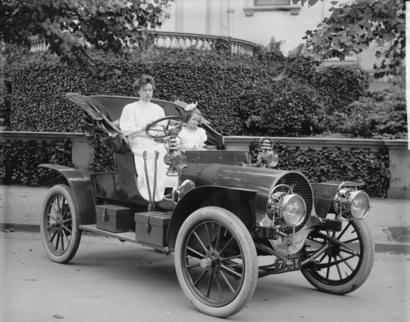
\includegraphics[width=\linewidth]{sample-franklin}
%  \caption{1907 Franklin Model D roadster. Photograph by Harris \&
%    Ewing, Inc. [Public domain], via Wikimedia
%    Commons. (\url{https://goo.gl/VLCRBB}).}
%  \Description{A woman and a girl in white dresses sit in an open car.}
% \end{figure}

\section{Benchmarks}


\subsection{Gregor's MNIST}

Gregors MNIST benchmark results are summarized in Table~\ref{tab:mnist}.

\begin{table*}[!ht]
\caption{Gregors MNIST Benchmarks}\label{tab:mnist}
    \centering
      \begin{adjustbox}{max width=\textwidth}
    \begin{tabular}{|l|l|l|l|l|l|l|l|l|l|}
    \hline
        Machine & real & user & sys & Driver & CUDA & GPU & \makecell{Date CPU \\released} & CPU & \makecell{Date CPU \\released} \\ \hline
        Gregors Machine & 0m11.534s & 0m13.914s & 0m05.186s & 510.47.03 & 11.6 & Gigabyte RTX3070 TI & May 31, 2021 & AMD 5950X & Nov 2020 \\ \hline
        Fox DGX & 0m19.987s & 5m12.991s & 0m49.266s & 450.142.00 & 11.0 & NVIDIA A100 80GB & & AMD EPYC 7742 64-Core & Aug 2019 \\ \hline
        Rivanna A100 & 0m29.263s & 0m14.585s & 0m7.399ss & 470.82.01 & 11.4 & NVIDIA A100-SXM4-40GB & May 14, 2020 & Intel(R) Xeon(R) CPU E5-2630 v3 @ 2.40GHz & Q3  2014 \\ \hline
        MacBook Pro & 0m31.01s & 0m25.26s & 130\% & N/A & N/A & N/A & N/A & M1 Max 66GB & Nov 2021 \\ \hline
        Rivanna P100 & 0m35.732s & 0m17.253s & 0m7.595s & 470.82.01 & 11.4 & Tesla P100-PCIE & & Intel(R) Xeon(R) CPU E5-2630 v3 @ 2.40GHz & Q3  2014 \\ \hline
        Rivanna V100 & 0m43.160s & 0m15.510s & 0m6.894s & 470.82.01 & 11.4 & Tesla V100-SXM2 & & Intel(R) Xeon(R) CPU E5-2630 v3 @ 2.40GHz & Q3  2014 \\ \hline
        Rivanna K80 & 0m57.588s & 0m20.322s & 0m9.612s & 470.82.01 & 11.4 & NVIDIA TESLA K80 & & Intel(R) Xeon(R) CPU E5-2630 v3 @ 2.40GHz & Q3  2014 \\ \hline
        Rivanna Frontend & 1m11.535s & 1m00.780s & 0m10.352s & N/A & N/A & N/A & & Intel(R) Xeon(R) CPU E5-2630 v3 @ 2.40GHz & Q3  2014 \\ \hline
    \end{tabular}
    \end{adjustbox}
\end{table*}

\subsection{Hardware}

\subsection{Aurora}
\label{id:anl} 

The Aurora supercomputer, sponsored by the U.S. Department of Energy (DOE), is part of the Argonne Leadership Computing Facility (ACLF). It was developed with the help of industry experts from Intel and Cray. Aurora offers HPC for data analytics and AI development with a peak performance of over 2 Exaflop DP. The system is based on the HPE Cray EX supercomputer platform and offers over 9,000 compute nodes.

Argonne National Laboratory (ANL), ... \cite{www-aurora}

\subsection{Summit}
\label{id:ornl} 

The Summit supercomputer, sponsored by the U.S. Department of Energy (DOE), is located in the Oak Ridge Leadership Computing Facility (OLCF). The open science computing system is available to government, academic, and industry researchers to solve complex problems in all fields of science. The system is powered by 4,608 nodes which each house multiple IBM POWER9 CPUs and NVIDIA Volta GPUs on top of half a terabyte of coherent memory.

Oak Ridge National Laboratory (ORNL), Summit \cite{www-summit}


\subsection{Perlmutter}
\label{id:nersc} 

The Perlmutter supercomputer, sponsored by the U.S. Department of Energy (DOE), is located in Shyh Wang Hall at Berkeley Lab and is operated by the National Energy Research Scientific Computing Center (NERSC). The supercomputer has a 12 cabinet GPU systems with over 1,500 nodes and a 12 cabinet CPU system containing over 3,000 nodes. It is supported by 35 petabytes of all-flash storage which can move data at 5 terabytes/sec.

National Energy Research Scientific Computing Center (NERSC), ...
\cite{www-perlmutter}

\subsection{SDSC}
\label{id:sdsc} 
\TODO{Which of the SDSC systems will we be benchmarking?}
San Diego Super Computing Center, ... \cite{www-expanse} 


\subsection{University of Virginia Rivanna}
\label{id:uva} 

UVA, Rivanna, A100, RTX3090, others may not have enough memory. 
\cite{www-rivanna}
\TODO{description of Rivanna on web page is not accurate.}

Containers are available on Rivanna through Singularity \cite{www-singularity} that can be loaded with modules \cite{www-modules}. We plan to utilize singularity, but target the formulation of the container in docker and than transform it to singularity. As singularity is installed also on other machines, we will leverage this deployment also on them. 

\begin{figure}[htb]
\resizebox{0.75\columnwidth}{!}{
\digraph{singularity}{
    node [shape=box style=rounded color=grey];
    Application -> GitHub
    "Dockerfile" -> "Docker Container" -> "Singularity Conversion" -> "Singularity Container" -> "Batch job (SLURM)"
}
}
\caption{Containerized Science Applications in Singularity}
\end{figure}

\subsection{Pearl}
\label{id:ral} 

The PEARL system, funded by the Alan Turing Institute, is hosted at the Rutherford Appleton Laboratory by the Science and Technology Facilities Council (STFC). It was developed for the advancement of AI and Machine Learning research with large-scale scientific datasets, already contributing to the fields of materials, environmental and life sciences, and astronomy. It is comprised of two NVIDIA DGX2 nodes, 32 GPUs, 3TB of system memory, 1TB of GPU memory, and 600TB of high-speed storage. 

Rutherford Appleton Laboratory (RAL), UK 
Pearl \cite{www-pearl-1}


\subsection {Nvidia DGX Workstation}
\label{id:dgx} 

The NVIDIA DGX Station A100 is a commercially available product that can provide powerful computing resources to all industries. The DGX Station is an AI resource that can run parallel jobs and support training, inference, and data analytics. It contains 4 NVIDIA A100 GPUs and up to 320 GBs of GPU memory. With the use of Multi-Instance GPU (MIG), each A100 GPU can be partitioned into 7 isolated instances.

DGX Fox \cite{www-dgx-station-a100}

\newcommand{\nvidia}[1]{
    \ifthenelse{\equal{#1}{A100}}{\href{https://www.nvidia.com/en-us/data-center/a100/}{NVIDIA #1}}{} 
    \ifthenelse{\equal{#1}{V100}}{\href{https://www.nvidia.com/en-us/data-center/a100/}{NVIDIA #1}}{}
    \ifthenelse{\equal{#1}{K80}}{\href{https://www.nvidia.com/en-gb/data-center/tesla-k80/}{NVIDIA #1}}{}
    \ifthenelse{\equal{#1}{P100}}{\href{https://www.nvidia.com/en-us/data-center/tesla-p100/}{NVIDIA #1}}{}
    \ifthenelse{\equal{#1}{RTX3090}}{\href{https://www.nvidia.com/en-us/geforce/graphics-cards/30-series/rtx-3090/}{NVIDIA #1}}{}
    \ifthenelse{\equal{#1}{RTX2080TI}}{\href{https://www.nvidia.com/en-us/data-center/tesla-p100/}{NVIDIA #1}}{}

%\newcommand{\nvidiaV}{\href{https://www.nvidia.com/en-us/data-center/v100/}{NVIDIA V100}}

\begin{table*}[htb]
    \caption{Overview of compute resources.}
    \label{tab:my_label}
    \centering
%\begin{adjustbox}{angle=90}
\begin{adjustbox}{max width=\textwidth}
    \begin{tabular}{|r|l|ll|r|l|l|l|l|l|}
        \hline
        Section & Organization   & Machine                         & & Processors    & GPUs             & \makecell{Memory\\/Device} &  \makecell{GPU\\/Device} & \makecell{No. of\\ nodes} & Commissioned \\ 
        \hline
        \hline
         \ref{id:anl}   & ANL    & Aurora & \cite{www-aurora}         &              &                  & & & &    ??? 2022   \\ \hline
         \ref{id:ornl}  & ORNL   & Summit &\cite{www-summit}         &        27000 & NVIDIA Volta     & & & &               \\ \hline
         \ref{id:nersc} & NERSC  & Perlmutter & \cite{www-perlmutter} &         6000 & \nvidia{A100}      & & & & Jan 2022      \\ \hline
         \ref{id:sdsc}  & SDSC   & Expanse & \cite{www-expanse}       &          200 & NVIDIA V100 SMX2 & & & &               \\ \hline
         \ref{id:uva}   & UVA    & Rivanna &\cite{www-rivanna}       &            8 & \nvidia{A100}      & 80GB & ? & &  Feb 2022      \\
            &    &  &       &            8 & \nvidia{A100}      & 40GB & 8 & &       \\
            &    &  &       &            ? & \nvidid{RTX3090}   & 24GB & ? & ? & 2021          \\
            &    &  &       &            ? & \nvidia{K80}       & 11GB & 8 & 9 & 2021          \\
            &    &  &       &            ? & \nvidia{V100}      & 16GB & 4 & 1 & 2021          \\
            &    &  &       &            ? & \nvidia{V100}      & 32GB & 4 & 12 & 2021          \\
            &    &  &       &            ? & \nvidia{P100}      & 12GB & 4 & 3 & 2021          \\
            &    &  &       &            ? & \nvidia{RTX2080TI} & 11GB & 10 & 2 & 2021          \\
         \hline
         \ref{id:ral}   & RAL    & Pearl &\cite{www-pearl-1}         &           16 & \nvidiaV      & & & &  \\ \hline
         \ref{id:dgx}   & Fox    & DGX Station A100 &\cite{www-dgx-station-a100} & 4 & \nvidiaA      & 80GB & 4 & 1 & May 2021      \\
         \hline
    \end{tabular}
    \end{adjustbox}
\end{table*}

Rivanna: \url{https://www.rc.virginia.edu/userinfo/rivanna/overview/}

\TODO{Add your personal computers to this table \url{https://github.com/Data-ScienceHub/mlcommons-science/issues/37}}
\begin{table*}[htb]
    \caption{Overview of compute resources.}
    \label{tab:my_label}
    \centering
%\begin{adjustbox}{angle=90}
\begin{adjustbox}{max width=\textwidth}
    \begin{tabular}{|r|l|l|r|l|l|l|l|l|}
        \hline
        Section & Organization   & Machine                         & Processors    & GPUs             & \makecell{Memory\\/Device} &  \makecell{GPU\\/Device} & \makecell{No. of\\ nodes} & Commissioned \\ 
        \hline
        \hline
         \ref{id:gcomputer}   & 
         Gregor    & 
         5950X   &  
         1 &   
         \href{https://www.gigabyte.com/Graphics-Card/GV-N307TGAMING-OC-8GD#kf}{GIGABYTE Gaming RTX 3070TI}  & 
         8GB & 
         1 & 
         1 & 
         Sep 2021   \\
            & 
            & 
            &  
            &   
         \href{https://rog.asus.com/us/graphics-cards/graphics-cards/rog-strix/rog-strix-rtx3090-o24g-gaming-model/}{ASUS ROG Strix RTX 3090} & 
         24GB & 
         1 & 
         1 & 
         Feb 2022   \\
         \hline
         \ref{id:tcomputer}   & Thomas.A  & i7-8750H &  1 &   NVIDIA GeForce RTX 2070 with Max-Q Design  & 16GB & 1 & 1 & 2019   \\
         \hline
         \ref{id:t2computer}   & Thomas.B  & i7-7700HQ &  1 &   NVIDIA GeForce GTX 1060  & 16GB & 1 & 1 & 2017   \\
         \hline
    \end{tabular}
    \end{adjustbox}
\end{table*}


\begin{acks}
\TODO{Geoffrey: please add acknowledgement for funding, other acks}
\end{acks}

\bibliographystyle{ACM-Reference-Format}
\bibliography{references}

\section*{Biographies}

\TODO{wrapfigure does somehow not work in this template}

{\bf Thomas Butler}
is a Graduate Student at University of Virginia's School of Data Science. His undergraduate degree is in Biomedical engineering. He has over 8 years of experience in the Infertility field helping patients, jointly running a Andrology lab, and contributing research to advance the field through joint research on how AMH effects pregnancy outcomes and sperm antibodies effect PSA. He has a certificate in Data Analytics from Georgia Institute of Technology.

{\bf Robert Knuuti}
is a Graduate Student at University of Virginia's School of Data Science. He has over 10 years experience in system architecture and software engineering, and specializes in Development Operations and Cloud Computing. He has constructed air gapped Continuous Integration and Continuous Delivery systems for multiple organizations each supporting more than 100 developers and has facilitated the construction of repeatable, tractable builds for users of these systems.

{\bf Jake Kolessar}
{is a Graduate Student at the University of Virginia's School of Data Science. He has a background in mechanical engineering and 2 years of experience as a Modeling, Simulation & Analysis Engineer. He has supported the software design and development of modeling capabilities for event simulation products as well as the integration of models into the simulation framework.}

{\bf Geoffrey C. Fox}
\TODO{Geoffery: fill out}


%\begin{wrapfigure}{r}{0.25\columnwidth}
%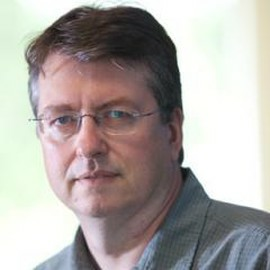
\includegraphics[width=0.24\columnwidth]{images/bio/gregor.png}
%\end{wrapfigure}

{\bf Gregor von Laszewski}
is a Research Professor at University of Virginia. He has more than 30 years of experience in parallel and distributed computing. Selected research organizations he worked in include NASA, Argonne National Laboratory, Indiana University. He is proud to have been contributing members of research teams that invented hybrid parallel genetic algorithms, Grid computing, and the first large scale academic hybrid cloud, as well as the larges scientific bibliometric analysis of XSEDE in the world.




\appendix

\section{Manuals Developed}

The following manuals have been developed by the team:

\begin{itemize}
    \item Introduction to Python \cite{las-intro-python}
\end{itemize}

\clearpage 

\section{Todo}

\subsection{Manual List}
\section{TODO and integrate}

Things to do: 

\begin{itemize}
    %% \item add presentation as cite,
    \item Review MLCommons \cite{www-mlcommons} 
    \item Use jabref \cite{www-jabrefg-org} for citation management
    \item Frequently check github \cite{www-mlcommons-eathquake}
    \item Read up on TFT \cite{www-onnen2021}
    \item Become familiar with the Attention Paper \cite{vaswani2017attention}
    \item Learn how to selfdeploy jupyterlab \cite{www-jupyterlab}
    \item Begin to learn about papermill \cite{www-papermill} \TODO{Rivanna's core configurations might be a bit limited on this front.  They do provide multiple versions of software (such as py2.7 and py3.8), but we may need to get permission to do something in userspace if we need to be very specific on a version of python.  Do we want to look into using tox, conda, or leave this up to the container ecosystem to solve?}
    \TODO{Gregor: add how to use conda and modules to switch python versions}
    \item virtualenv on rivanna for a particular python version.
    \item depends on Tensorflow
    \TODO{Below this line are objectives or targets to take the current modeling solution and mature it for other platforms / ecosystems.  Rivanna uses Lua's lmod ecosystem for jailing a process, and anaconda uses solved environments for dependencies that extend beyond just python modules.}
    \item Familiarize yourself with Rivanna's modules \cite{www-modules}  and conda \cite{www-conda} environments.
    \item pytorch \cite{www-pytorch}
    \TODO{There is interest in comparing pytorch and tensoflow}
    \item horovod \cite{www-horovod}
    \TODO{MLCommons project that can target a few platforms using a YAML contract.  Once we solve the target environment, we can likely target porting this way.}
    
    \item \mlcube{} \cite{www-mlcube} 
\end{itemize}


\subsection{Generated List}
\listoftodos{}

To find a general list of todo actions, consult

\begin{itemize}
\item The \href{https://github.com/cybertraining-dsc/capstone-eartquake/blob/main/TODO.md}{TODO.md} 
\item The \href{https://github.com/Data-ScienceHub/mlcommons-science/projects/1}{GitHub Project}
\end{itemize}

\section{Progress Reports}

\subsection{Progress Report A}

Dates covered: Jan 27 - Feb 23rd

Due: Feb 24th, 2022

\begin{itemize}
\item Reviewed background information \footnote{\url{https://github.com/Data-ScienceHub/mlcommons-science/issues/1}}
    \begin{itemize}
    \item Earthquake Nowcasting with Deep Learning
    \item MLCommons Benchmark Presentation
    \item Attention is ALl you Need
    \item MLCommons TEvolOp Earthquake Forcasting objectives
    \item Learning on Temporal Fusion Transformers
    \item MLCommons and AI for Science illustrated by Deep Learning for Geospatial Time Series
    \end{itemize}
\item Reviewed background technologies \footnote{\url{https://github.com/Data-ScienceHub/mlcommons-science/issues/2}}
    \begin{itemize}
    \item lmod - lua module and environment management (used on rivanna)
    \item pip / conda env - python package management
    \item SLURM - an HPC batch job runner
    \item papermill - parameterized jupyter notebooks
    \item horovod - distributed framework for running multiple deep learning frameworks
    \item \mlcube{} - MLCommons repeatable machine learning framework with multiple backends.
    \item singularity - container runtimes targeting HPC clusters
    \item docker
\end{itemize}
\item Wrote introduction to paper (in progress) \footnote{\url{https://www.overleaf.com/project/61f1e28f076f4111c3ba927e}}
    \begin{itemize}
    \item added references to references.bib in overleaf
    \end{itemize}
\item Revised Intro to Python guide for conda installations so it doesn't interfere with pyenv or other shell commands.\footnote{\url{https://github.com/cloudmesh-community/book/pull/574}} \footnote{\url{https://github.com/cloudmesh-community/book/pull/575}}
\item Solved conda environment and requirements.txt for colab notebook
\footnote{\url{https://github.com/Data-ScienceHub/mlcommons-science/issues/12}} \footnote{\url{https://github.com/laszewsk/mlcommons/pull/1}} \footnote{\url{https://github.com/laszewsk/mlcommons/pull/3}}
\item build docker container image that can run python 3.9.7 and conda
\item verified access to GPU allocations in Rivanna
\end{itemize}

\subsection{Progress Report B}

Dates covered: Feb 24th - Mar 23rd

Due: Mar 24th, 2022

\subsection{Presentation}

Dates covered: Mar 24th - April 27th

Due: April 28th, 2022




\end{document}
\endinput
%%
%% End of file `sample-sigplan.tex'.
